\documentclass[english,t]{beamer}
%\documentclass[finnish,english,handout]{beamer}

\usepackage[T1]{fontenc}
\usepackage[utf8]{inputenc}
\usepackage{newtxtext} % times
%\usepackage[scaled=.95]{cabin} % sans serif
\usepackage{amsmath}
\usepackage[varqu,varl]{inconsolata} % typewriter
\usepackage[varg]{newtxmath}
\usefonttheme[onlymath]{serif} % beamer font theme
\usepackage{microtype}
\usepackage{url}
\urlstyle{same}

\mode<presentation>
{
  \setbeamercovered{invisible}
  \setbeamertemplate{itemize items}[circle]
  \setbeamercolor{frametitle}{bg=white,fg=navyblue}
  \setbeamertemplate{navigation symbols}{}
  \setbeamertemplate{headline}[default]{}
  \setbeamertemplate{footline}[split]
% Uncomment if want to show notes
%\setbeameroption{show notes}
}

\pdfinfo{            
  /Title      (BDA, Lecture 1, Practicalities) 
  /Author     (Aki Vehtari) % 
  /Keywords   (Bayesian data analysis)
}

\definecolor{navyblue}{rgb}{0,0,0.5}
% \definecolor{midnightblue}{rgb}{0.0977,0.0977,0.4375}
% \definecolor{lightgray}{rgb}{0.95,0.95,0.95}
% \definecolor{section}{rgb}{0,0.2549,0.6784}
% \definecolor{list1}{rgb}{0,0.2549,0.6784}
% \renewcommand{\emph}[1]{\textcolor{navyblue}{#1}}

\DeclareMathOperator{\E}{E}
\DeclareMathOperator{\Var}{Var}
\DeclareMathOperator{\var}{var}
\DeclareMathOperator{\Sd}{Sd}
\DeclareMathOperator{\sd}{sd}
\DeclareMathOperator{\Bin}{Bin}
\DeclareMathOperator{\Beta}{Beta}
\DeclareMathOperator{\logit}{logit}
\DeclareMathOperator{\N}{N}
\DeclareMathOperator{\U}{U}
\DeclareMathOperator{\BF}{BF}
%\DeclareMathOperator{\Pr}{Pr}
\def\euro{{\footnotesize \EUR\, }}
\DeclareMathOperator{\rep}{\mathrm{rep}}


\title[]{Bayesian data analysis}
\subtitle{Practical matters}

\author{Aki Vehtari}

\institute[Aalto University]{}

\begin{document}

\begin{frame}
  \frametitle{Bayesian data analysis (Aalto fall 2024)}  %
  \framesubtitle{Practical matters}
  
  \begin{itemize}
  \item Book: Gelman, Carlin, Stern, Dunson, Vehtari \& Rubin: Bayesian Data
    Analysis, Third Edition. {\footnotesize (online PDF available)}
  \item The course website has more detailed information\\
    {\small\url{https://avehtari.github.io/BDA_course_Aalto/Aalto2024.html}}
  \item Timetable: see the course website
  \item TAs: David Kohns, Mélanie Guhl, Noa Kallioinen, Anna Riha, Varun Shanmugam, Maksim Sinelnikov, Teemu
    Säilynoja
    \end{itemize}
    \vspace{-0.5\baselineskip}
 \begin{center}
   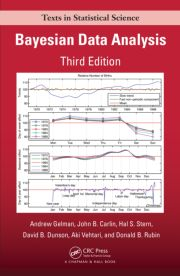
\includegraphics[width=2.6cm]{figs/BDA3.jpg}
 \end{center}

\end{frame}

\begin{frame}

  \frametitle{Bayesian data analysis}  %
  \framesubtitle{Schedule}

  \begin{itemize}
  \item No lecture on 9th September as I and most TAs are in StanCon conference
  \item Yes lecture on 14th October although it is evaluation week
  \item No lecture on 24th October
  \item Project presentations on week starting 9th December
  \end{itemize}
  
\end{frame}

\begin{frame}
  \frametitle{Bayesian data analysis}  %
  \framesubtitle{prerequisites}
  \begin{itemize}
  \item Basic terms of probability theory
    \begin{itemize}
    \item probability, probability density, distribution
    \item sum, product rule, and Bayes' rule
    \item expectation, mean, variance, median
    \end{itemize}
  \item Some algebra and calculus
  \item Basic visualization techniques (R or Python)
    \begin{itemize}
    \item histogram, density plot, scatter plot
    \end{itemize}
  \end{itemize}

  These will be tested with the first assignment round

\end{frame}

\begin{frame}
  \frametitle{Bayesian data analysis}  %
  \framesubtitle{prerequisites}
  \begin{itemize}
  \item What to do if the course seems to be too difficult
    \begin{itemize}
    \item refresh your memory on prerequisites (see the course web
      site for some links)
    \item ask for help
    \item consider reading Regression and Other Stories \url{https://avehtari.github.io/ROS-Examples/}
    \item consider reading Statistical rethinking + watching videos \url{https://xcelab.net/rm/statistical-rethinking/}
    \end{itemize}
  \end{itemize}

\end{frame}

\begin{frame}
  \frametitle{Bayesian data analysis}  %
  \framesubtitle{Course contents}
  \begin{itemize}
  \item Background (Ch 1)
  \item Model, likelihood, prior, posterior, integration (Ch 2)
  \item Integration in multiparameter models (Ch 3)
  \item Basic integration methods (Ch 10)
  \item Markov chain Monte Carlo integration (Ch 11--12)
  \item Stan and probabilistic programming
  \item Hierarchical models (Ch 5)
  \item Model checking (Ch 6)
  \item Evaluating and comparing models (Ch 7 + extra material)
  \item Decision analysis (Ch 9)
  \item Large sample properties and Laplace approximation (Ch 4)
  \item Bayesian workflow (project)
  \end{itemize}
  
\end{frame}


\begin{frame}
  \frametitle{Bayesian data analysis}  %
  \framesubtitle{Different learning styles}

  \begin{itemize}
  \item Reading
  \item Listening lectures
  \item Solving problems
    \begin{itemize}
    \item mathematical derivations
    \item programming
    \end{itemize}
  \end{itemize}
  
\end{frame}

\begin{frame}
  \frametitle{Bayesian data analysis}  %
  \framesubtitle{Assessment}
    \begin{itemize}
    \item Assignments 40\%
    \item E-exam 10\%
    \item Project work and presentation 50\%\\~
    \item Minimum of 50\% of points must be obtained from each
    \end{itemize}

\end{frame}

\begin{frame}
  \frametitle{Bayesian data analysis}  %

  \begin{itemize}
  \item Lectures describe basics and give broader overview (recorded
    and made available)
    \begin{itemize}
    \item written material has all the details and self-study
      is possible
    \end{itemize}
  \item Supporting material and assignments in
    {\small\url{https://avehtari.github.io/BDA_course_Aalto/Aalto2024.html}}
    \begin{itemize}
    \item reading instructions and chapter notes
    \item demos (very useful for assignments)
    \item slides (not very useful without the lectures)
    \item video clips
    \item links to additional material
    \end{itemize}
   \item R demos {\small\url{https://avehtari.github.io/BDA_course_Aalto/demos.html\#BDA_R_demos}}
  \item (Python demos {\small\url{https://avehtari.github.io/BDA_course_Aalto/demos.html\#BDA_Python_demos})}
  \item Aalto Zulip chat instance (link in MyCourses)
  \end{itemize}

\end{frame}

\begin{frame}
  \frametitle{Bayesian data analysis}  %
  \framesubtitle{Assignments}
  \begin{itemize}
  \item Weekly assignments (some have two weeks time)
    \begin{itemize}
    \item R simulation assignments
    \item Stan probabilistic programming assignments (via R)
    \end{itemize}
  \item Related R demos available (see the course web site)
  \item TAs available: the web page for TA session times
  \item Assignment deadlines on Sunday (see detailed info in the course web page)
    \begin{itemize}
    \item we recommend to submit before Friday 3pm as TAs are not
      available during the weekend
    \item we allow the late submission on Sunday as some students are
      working on weekdays
    \end{itemize}
  \item Submit assignment answers via MyCourses Quizzes
    \begin{itemize}
    \item autosubmission of Quiz answers at the deadline time
    \end{itemize}
  \item For some later assignments submit also a report in FeedbackFruits
  % \item After the assignment deadline, the grading period Monday--Tuesday
  % \item Students grade 3 other assignments using peergrade.io
  \end{itemize}
  
\end{frame}

\begin{frame}
  \frametitle{Bayesian data analysis}  %
  \framesubtitle{R}

  \begin{itemize}
  \item We use R in the course as there are more packages for Stan and
    statistical analysis in general in R
    \begin{itemize}
    \item this will make specifically it easier to work with
      hierarchical models in the later part of the course
    \end{itemize}
  \end{itemize}
  
\end{frame}

\begin{frame}
  \frametitle{Bayesian data analysis}  %
  \framesubtitle{Assignments}
  \begin{itemize}
  \item Assignments are available in the course website
  \item Assignments are returned by answering MyCourses Quizzes and in some
    later rounds also by submitting to FeedbackFruits
  \end{itemize}
\end{frame}

\begin{frame}
  \frametitle{Assignments}  %
  \framesubtitle{MyCourses Quizzes}
  \begin{itemize}
  \item Assignment answerd submitted via MyCourses Quizzes
    \begin{itemize}
    \item multiple choice questions
    \item multiresponse questions
    \item numerical value questions (with tolerance)
    \end{itemize}
  \end{itemize}
\end{frame}

\begin{frame}
  \frametitle{Assignments}  %
  \framesubtitle{FeedbackFruits}
  \begin{itemize}
  \item Peergrading used in BDA course since 2016
    \begin{itemize}
    \item peergrade.io used 2016--2023, but it was shut down in 2023
    \item FeedbackFruits is missing some features, and that's why we
      use it only for some assignments and for the project report
    \end{itemize}
  \item Submit report as PDF
  \item Each student grades 3 assignment reports (randomly distributed)
  \item Detailed grading instructions -- rubric (available also on the course website)
  \item Graders provide also text feedback
  \item Quality of grading is evaluated, too
  \item See more at
    \url{https://avehtari.github.io/BDA_course_Aalto/assignments.html}
    \begin{itemize}
    \item FeedbackFruits instructions still in progress
    \end{itemize}
  \end{itemize}
  
\end{frame}

\begin{frame}
  \frametitle{Assignments}  %
  \framesubtitle{Feedbackfruits}

  \begin{itemize}
  \item Login with Aalto account
  \item Combined score: 90\% submission performance, 10\% feedback performance
    % \pause
  % \item Hand-in score:
  %   \begin{itemize}
  %   \item averaging the scores from peers
  %   \item after flagging, teacher may overrule the score
  %   \item different assignments have different weights
  %   \end{itemize}
  %   See details at \url{http://help.peergrade.io/interfaces-and-features/grading-and-scores/the-hand-in-score}
  %   \pause
  % \item Feedback score:
  %   \begin{itemize}
  %   \item When students receive a review, they are asked to react to
  %     it using a scale ranging from ``Not useful at all'' to ``Extremely
  %     useful''.
  %   \item These ratings each correspond to a score between 0\% and 100\%.
  %   \item The feedback score is the average of the reaction scores.
  %   \item ``Somewhat useful. Could be more elaborate.'' is the
  %     baseline reaction.
  %   \end{itemize}
  \end{itemize}
  
\end{frame}

% \begin{frame}
%   \frametitle{FeedbackFruits}  %
%   \framesubtitle{Registration}
%   \begin{itemize}
%   \item Go to BDA MyCourses page
%   \item Click Peergrade and login with Aalto account
%   \end{itemize}
  
% \end{frame}

\begin{frame}
  \frametitle{Assignments}  %
  \framesubtitle{Plagiarism and empty reports}
  \begin{itemize}
  \item It's OK to discuss assignments with others
  \item It's OK to use code from the demos (mention the source)
  \item It's OK to use AI, but need to mention when and how used
    \begin{itemize}
    \item Warning: I have tested these and they can provide very vague
      or completely wrong results for the course contents
    \item Might be most useful for getting ideas for code and markdown syntax
    \end{itemize}
  \item Don't copy reports from others or from internet
  \item Don't submit empty, almost empty or nonsense report
    \begin{itemize}
    \item these will be problematic for other students
    \item if you see such, send TAs a message and mark it as
      problematic in Peergrade and get another one for grading
    \end{itemize}
  \end{itemize}
  
\end{frame}

\begin{frame}
  \frametitle{E-exam}  %
  \begin{itemize}
  \item All exam questions picked from the assignment questions
  \item No programming tasks
  \item Choose your own time to take the e-exam %from 18 November to 13 December
  \end{itemize}
  
\end{frame}


\begin{frame}
  \frametitle{Project work}  %
  \framesubtitle{}
  \begin{itemize}
  \item Project work in groups of 1--3
    \begin{itemize}
    \item combines all the pieces learned in one project work
    \item Quarto notebook report
    \item project report peer graded (30\% of the project score)
    \item oral presentation graded by me and TAs (70\% of the project score)
    \end{itemize}
  \item More about projects later
  \end{itemize}
  
\end{frame}

\begin{frame}

  \frametitle{Zulip chat}  %
  \framesubtitle{bda2024.zulip.aalto.fi}

  \begin{itemize}
  \item Aalto login, hosted by Aalto IT, deleted after one year
  \item The web interface is better\\ (the mobile app has push
    notifications capability, but Aalto has not enabled it in Aalto
    server)
  \item Different streams for announcements, general, assignments, etc.
  \end{itemize}
  
\end{frame}

\begin{frame}

  \frametitle{RStudio, Quarto, R markdown}  %
  \framesubtitle{}

  \begin{itemize}
  \item RStudio is a great IDE for R
  \item Quarto is a markdown language for making reports mixing
    text, code, equations, tables, etc
    \begin{itemize}
    \item \textit{Quarto is the next iteration of R Markdown, and
        allows you can create dynamic content with Python, R, Julia,
        and Observable, author documents as plain text markdown or
        Jupyter notebooks, and output to multiple format types.}
    \end{itemize}
  \item RStudio has also visual editor for Quarto (and R markdown)
    making it easy for new users
  \item RStudio is also installed in Aalto JupyterHub
  \end{itemize}
  
\end{frame}  

\begin{frame}

  \frametitle{jupyter.cs.aalto.fi}  %
  \framesubtitle{}

  \begin{itemize}
  \item No need to install anything locally, everything can be done in
    Aalto JupyterHub
    \begin{itemize}
    \item The \textbf{notebooks} folder is the only persistent folder
      (stays there if you sign out) so save everything to that folder!
    \item You may access JupyterHub folder as a network drive by SMB
      mounting it on your own computer
    \item See more in the course FAQ
    \end{itemize}
  \item There is some support for local installations (see FAQ in the
    course web page)
  \end{itemize}
  
\end{frame}  

\begin{frame}

  \frametitle{FAQ}  %
  \framesubtitle{}

  \begin{itemize}
  \item {\small\url{https://avehtari.github.io/BDA_course_Aalto/FAQ.html}}
  \item For example,
    \begin{itemize}
    \item R packages used in demos
    \item Installing aaltobda package
    \item Installation problems
    \item Remote access
    \item Tidyverse and pipes
    \item What if I missed some deadline or wasn’t able to do some part of the course
    \end{itemize}
  \end{itemize}
  
\end{frame}  

\end{document}

%%% Local Variables:
%%% mode: latex
%%% TeX-master: t
%%% End:
